\section{Casos de uso}\label{cap:casos_de_uso}

Los casos de uso son los escenarios detallados que describen cómo interactúan los diferentes usuarios con la aplicación, desde la consulta de información hasta la gestión administrativa de la Semana Santa. Debido a que los usuarios pueden comportarse con diferentes roles (ciudadano, cofrade, Junta de Cofradías o administrador), es importante diferenciar los casos de uso entre cada uno de ellos. Para ello se han dividido los mismos en cuatro diagramas (ver figuras ~\ref{fig:casoUso1}, ~\ref{fig:casoUso2}, ~\ref{fig:casoUso3}, ~\ref{fig:casoUso4}), uno para cada rol.

\begin{figure}[H]
    \centering
    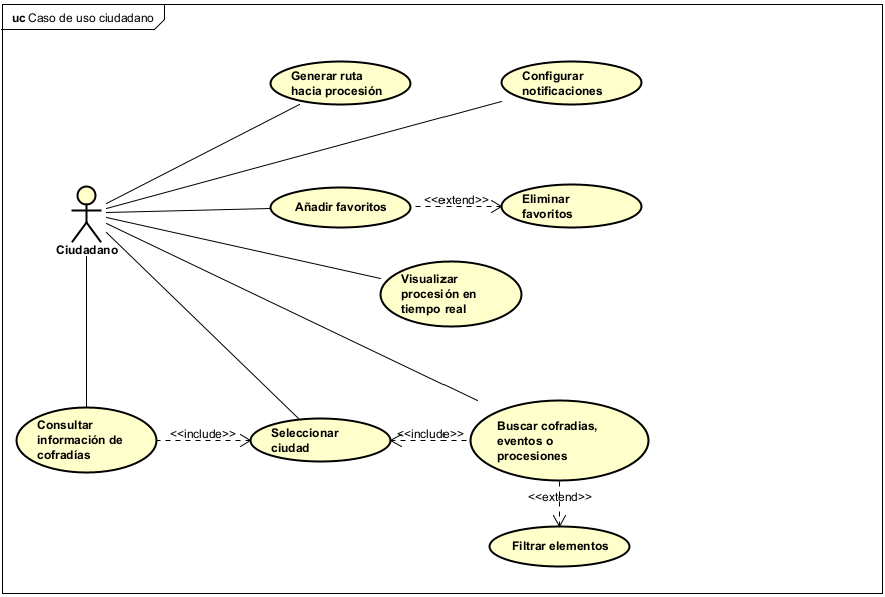
\includegraphics[width=0.6\textwidth]{imagenes/casoDeUsoCiudadano.png}
    \caption{Diagrama de caso de uso Ciudadano}
    \label{fig:casoUso1}
\end{figure}

\begin{figure}[H]
    \centering
    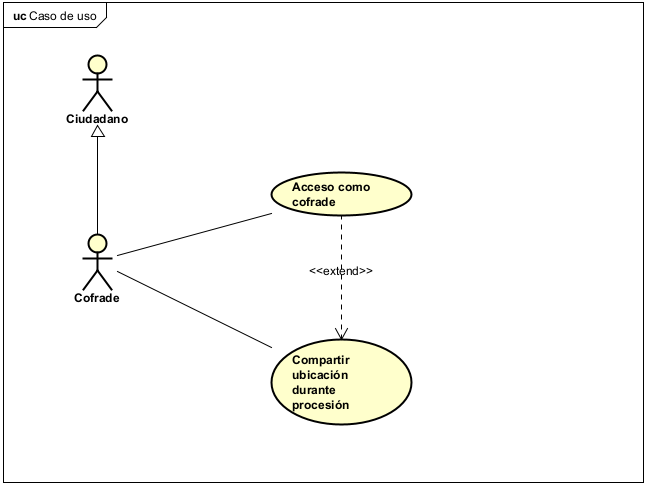
\includegraphics[width=0.6\textwidth]{imagenes/casoDeUsoCofrade.png}
    \caption{Diagrama de caso de uso Cofrade}
    \label{fig:casoUso2}
\end{figure}

\begin{figure}[H]
    \centering
    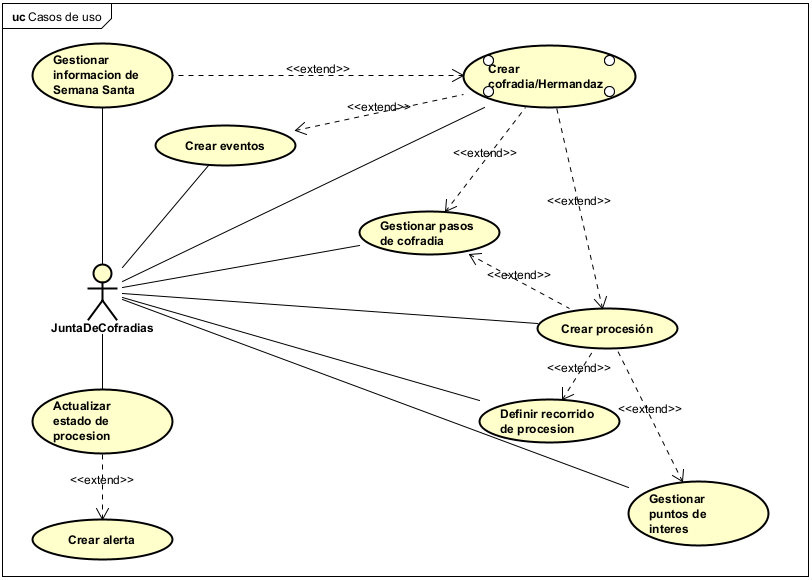
\includegraphics[width=0.6\textwidth]{imagenes/casoDeUsoJuntaDeCofradias.png}
    \caption{Diagrama de caso de uso Junta de Cofradías}
    \label{fig:casoUso3}
\end{figure}


\begin{figure}[H]
    \centering
    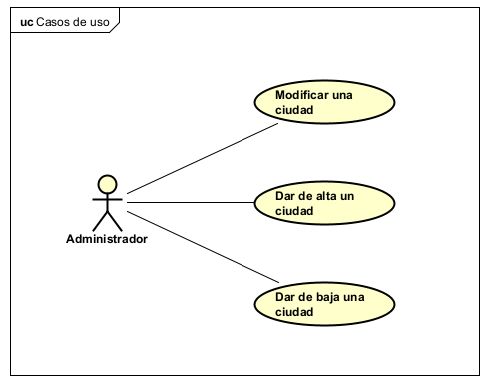
\includegraphics[width=0.6\textwidth]{imagenes/casoDeUsoAdministrador.png}
    \caption{Diagrama de caso de uso Administrador}
    \label{fig:casoUso4}
\end{figure}

En las siguientes tablas se exponen los cinco casos de uso más representativos del sistema, uno por cada rol implicado (ciudadano, cofrade, Junta de Cofradías y administrador), donde se detallan: el caso de uso, los actores que lo realizan, las precondiciones necesarias para iniciar el caso de uso, las postcondiciones que deben cumplirse al completarse, una secuencia base de pasos, secuencias alternativas que pueden darse durante la ejecución y los requisitos relacionados con el caso de uso. El resto de los casos de uso identificados, de carácter más secundario, se recogen en el Apéndice~\ref{cap:casos_de_uso_adicionales}.


\begin{table}[h!]
    \centering
    \renewcommand{\arraystretch}{1.5}

    \begin{tabular}{|p{4cm}|p{11cm}|}
        \hline
        \multicolumn{2}{|l|}{\textbf{Caso de uso: Visualizar procesión en tiempo real}}                                                             \\
        \hline
        \textbf{Resumen}                                                                                                                           & El usuario visualiza la posición actual de una procesión en el mapa. \\
        \hline
        \textbf{Actor}                                                                                                                             & Ciudadano                                                            \\
        \hline
        \textbf{Precondición}                                                                                                                      & La procesión está en curso El usuario tiene conexión a internet      \\
        \hline
        \textbf{Postcondición}                                                                                                                     & Se muestra la lista de cofradías con su información.                 \\
        \hline
        \multicolumn{2}{|l|}{\textbf{Secuencia Base}}                                                                                               \\
        \hline
        \multicolumn{2}{|p{15cm}|}{ [1] El usuario selecciona una procesión activa. }                                                               \\
        \hline
        \multicolumn{2}{|p{15cm}|}{ [2] El sistema muestra el mapa con el recorrido de la procesión. }                                              \\
        \hline
        \multicolumn{2}{|p{15cm}|}{ [3] El sistema actualiza la posición en tiempo real. }                                                          \\
        \hline
        \multicolumn{2}{|p{15cm}|}{ [4] El usuario puede interactuar con el mapa (zoom, desplazamiento). }                                          \\
        \hline
        \multicolumn{2}{|l|}{\textbf{Secuencia Alternativa}}                                                                                        \\
        \hline
        \multicolumn{2}{|p{15cm}|}{ [1.a.1] La procesión no está activa: El sistema muestra el recorrido planificado sin posición en tiempo real. } \\
        \hline
        \multicolumn{2}{|p{15cm}|}{ [3.a.1] Pérdida de conexión: El sistema muestra la última posición conocida. }                                  \\
        \hline
        \textbf{Requisitos Relacionados}                                                                                                           & RF-05, RF-14 y RF-16.                                                \\
        \hline
    \end{tabular}
    \caption{Caso de uso: Visualizar procesión en tiempo real}
\end{table}


\begin{table}[h!]
    \centering
    \renewcommand{\arraystretch}{1.5}

    \begin{tabular}{|p{4cm}|p{11cm}|}
        \hline
        \multicolumn{2}{|l|}{\textbf{Caso de uso: Compartir ubicación durante procesión}}                                                   \\
        \hline
        \textbf{Resumen}                                                                                                                   & Un cofrade comparte su ubicación en tiempo real durante una procesión.                                         \\
        \hline
        \textbf{Actor}                                                                                                                     & Cofrade                                                                                                        \\
        \hline
        \textbf{Precondición}                                                                                                              & El cofrade está registrado, el cofrade tiene permisos de ubicación y hay una procesión de su cofradía en curso \\
        \hline
        \textbf{Postcondición}                                                                                                             & La ubicación del cofrade se transmite al sistema.                                                              \\
        \hline
        \multicolumn{2}{|l|}{\textbf{Secuencia Base}}                                                                                       \\
        \hline
        \multicolumn{2}{|p{15cm}|}{ [1] El cofrade accede a la procesión activa de su cofradía. }                                           \\
        \hline
        \multicolumn{2}{|p{15cm}|}{ [2] El cofrade activa la opción de compartir ubicación. }                                               \\
        \hline
        \multicolumn{2}{|p{15cm}|}{ [3] El sistema solicita permisos de ubicación si no los tiene. }                                        \\
        \hline
        \multicolumn{2}{|p{15cm}|}{ [4] El cofrade concede los permisos. }                                                                  \\
        \hline
        \multicolumn{2}{|p{15cm}|}{ [5] El sistema comienza a transmitir la ubicación. }                                                    \\
        \hline
        \multicolumn{2}{|p{15cm}|}{ [6] El sistema muestra indicador de ubicación compartida. }                                             \\
        \hline
        \multicolumn{2}{|l|}{\textbf{Secuencia Alternativa}}                                                                                \\
        \hline
        \multicolumn{2}{|p{15cm}|}{ [4.a.1] El usuario deniega permisos: El sistema informa que no puede compartir ubicación sin permiso. } \\
        \hline
        \multicolumn{2}{|p{15cm}|}{ [2.a.1] Cancelación de la operación: El usuario desea cancelar la operacion. }                             \\
        \hline
        \multicolumn{2}{|p{15cm}|}{ [5.a.1] Pérdida de conexión: El sistema muestra la última posición conocida. }                          \\
        \hline
        \textbf{Requisitos Relacionados}                                                                                                   & RF-13 y RF-17.                                                                                                 \\
        \hline
    \end{tabular}
    \caption{Caso de uso: Compartir ubicación durante procesión}
\end{table}


\begin{table}[h!]
    \centering
    \renewcommand{\arraystretch}{1.5}

    \begin{tabular}{|p{4cm}|p{11cm}|}
        \hline
        \multicolumn{2}{|l|}{\textbf{Caso de uso: Crear alerta}}                                                         \\
        \hline
        \textbf{Resumen}                                                                                                & La Junta de Cofradías crea una alerta para informar a los usuarios sobre incidencias o información relevante. \\
        \hline
        \textbf{Actor}                                                                                                  & Junta de Cofradías                                                                                            \\
        \hline
        \textbf{Precondición}                                                                                           & El usuario tiene rol de Junta de Cofradías.                                                                   \\
        \hline
        \textbf{Postcondición}                                                                                          & La alerta queda creada y se envian notificaciones a los usuarios afectados.                                   \\
        \hline
        \multicolumn{2}{|l|}{\textbf{Secuencia Base}}                                                                    \\
        \hline
        \multicolumn{2}{|p{15cm}|}{ [1] El usuario accede al panel de gestion de alertas. }                              \\
        \hline
        \multicolumn{2}{|p{15cm}|}{ [2] El usuario selecciona crear nueva alerta. }                                      \\
        \hline
        \multicolumn{2}{|p{15cm}|}{ [3] El sistema muestra el formulario de creacion. }                                  \\
        \hline
        \multicolumn{2}{|p{15cm}|}{ [4] El usuario selecciona el tipo de alerta. }                                       \\
        \hline
        \multicolumn{2}{|p{15cm}|}{ [5] El usuario introduce titulo y mensaje de la alerta. }                            \\
        \hline
        \multicolumn{2}{|p{15cm}|}{ [6] El usuario selecciona la prioridad de la alerta. }                               \\
        \hline
        \multicolumn{2}{|p{15cm}|}{ [7] El usuario define fecha de expiracion (opcional). }                              \\
        \hline
        \multicolumn{2}{|p{15cm}|}{ [8] El usuario selecciona los destinatarios. }                                       \\
        \hline
        \multicolumn{2}{|p{15cm}|}{ [9] El usuario confirma la creacion. }                                               \\
        \hline
        \multicolumn{2}{|p{15cm}|}{ [10] El sistema crea la alerta y envia notificaciones. }                             \\
        \hline
        \multicolumn{2}{|l|}{\textbf{Secuencia Alternativa}}                                                             \\
        \hline
        \multicolumn{2}{|p{15cm}|}{ [4.a.1] Cancelación de la operación: El usuario desea cancelar la operacion. }          \\
        \hline
        \multicolumn{2}{|p{15cm}|}{ [5.a.1] Cancelación de la operación: El usuario desea cancelar la operacion. }          \\
        \hline
        \multicolumn{2}{|p{15cm}|}{ [6.a.1] Cancelación de la operación: El usuario desea cancelar la operacion. }          \\
        \hline
        \multicolumn{2}{|p{15cm}|}{ [7.a.1] Cancelación de la operación: El usuario desea cancelar la operacion. }          \\
        \hline
        \multicolumn{2}{|p{15cm}|}{ [8.a.1] Cancelación de la operación: El usuario desea cancelar la operacion. }          \\
        \hline
        \multicolumn{2}{|p{15cm}|}{ [9.a.1] Datos incompletos: El sistema muestra los campos requeridos. }               \\
        \hline
        \multicolumn{2}{|p{15cm}|}{ [10.a.1] Error al enviar notificaciones: El sistema reintenta y registra el error. } \\
        \hline
        \textbf{Requisitos Relacionados}                                                                                & RF-11, RF-12 y RF-26.                                                                                         \\
        \hline
    \end{tabular}
    \caption{Caso de uso: Crear alerta}
\end{table}

\begin{table}[h!]
    \centering
    \renewcommand{\arraystretch}{1.5}

    \begin{tabular}{|p{4cm}|p{11cm}|}
        \hline
        \multicolumn{2}{|l|}{\textbf{Caso de uso: Acceso como cofrade}}                                                                   \\
        \hline
        \textbf{Resumen}                                                                                                                 & Un usuario se registra en la aplicación como miembro de una cofradía. \\
        \hline
        \textbf{Actor}                                                                                                                   & Cofrade                                                               \\
        \hline
        \textbf{Precondición}                                                                                                            & El usuario no está registrado.                                        \\
        \hline
        \textbf{Postcondición}                                                                                                           & El usuario queda registrado y puede acceder a funciones de cofrade.   \\
        \hline
        \multicolumn{2}{|l|}{\textbf{Secuencia Base}}                                                                                     \\
        \hline
        \multicolumn{2}{|p{15cm}|}{ [1] El usuario selecciona la opción de registro. }                                                    \\
        \hline
        \multicolumn{2}{|p{15cm}|}{ [2] El sistema muestra el formulario de registro (Introducir código de acceso para dicha cofradía). } \\
        \hline
        \multicolumn{2}{|p{15cm}|}{ [3] El usuario introduce el código de acceso de la cofradía. }                                        \\
        \hline
        \multicolumn{2}{|p{15cm}|}{ [4] El sistema valida el código. }                                                                    \\
        \hline
        \multicolumn{2}{|p{15cm}|}{ [5] El sistema muestra mensaje informando del correcto acceso. }                                      \\
        \hline
        \multicolumn{2}{|l|}{\textbf{Secuencia Alternativa}}                                                                              \\
        \hline
        \multicolumn{2}{|p{15cm}|}{ [3.a.1] Cancelación de la operación: El usuario desea cancelar la operacion. }                           \\
        \hline
        \multicolumn{2}{|p{15cm}|}{ [5.a.1] Codigo inválido: El sistema muestra los errores de validación. }                              \\
        \hline
        \textbf{Requisitos Relacionados}                                                                                                 & RF-02.                                                                \\
        \hline
    \end{tabular}
    \caption{Caso de uso: Acceso como cofrade}
\end{table}

\begin{table}[h!]
    \centering
    \renewcommand{\arraystretch}{1.5}

    \begin{tabular}{|p{4cm}|p{11cm}|}
        \hline
        \multicolumn{2}{|l|}{\textbf{Caso de uso: Dar de alta ciudad}}                                                      \\
        \hline
        \textbf{Resumen}                                                                                                    & El administrador da de alta una nueva ciudad disponible en la aplicación.                                            \\
        \hline
        \textbf{Actor}                                                                                                      & Administrador                                                                                                         \\
        \hline
        \textbf{Precondición}                                                                                               & El usuario tiene rol de Administrador.                                                                               \\
        \hline
        \textbf{Postcondición}                                                                                              & La nueva ciudad queda disponible en el sistema.                                                                      \\
        \hline
        \multicolumn{2}{|l|}{\textbf{Secuencia Base}}                                                                       \\
        \hline
        \multicolumn{2}{|p{15cm}|}{ [1] El usuario accede al panel de administración. }                                     \\
        \hline
        \multicolumn{2}{|p{15cm}|}{ [2] El sistema muestra la lista de ciudades existentes. }                               \\
        \hline
        \multicolumn{2}{|p{15cm}|}{ [3] El usuario selecciona la opción de añadir ciudad. }                                 \\
        \hline
        \multicolumn{2}{|p{15cm}|}{ [4] El usuario introduce los datos de la nueva ciudad. }                                \\
        \hline
        \multicolumn{2}{|p{15cm}|}{ [5] El sistema valida y guarda la nueva ciudad. }                                       \\
        \hline
        \multicolumn{2}{|l|}{\textbf{Secuencia Alternativa}}                                                                \\
        \hline
        \multicolumn{2}{|p{15cm}|}{ [4.a.1] Cancelación de la operación: El usuario desea cancelar la operación. }          \\
        \hline
        \multicolumn{2}{|p{15cm}|}{ [5.a.1] Datos incompletos: El sistema muestra los campos requeridos. }                  \\
        \hline
        \textbf{Requisitos Relacionados}                                                                                    & RF-26.                                                                                                                \\
        \hline
    \end{tabular}
    \caption{Caso de uso: Dar de alta ciudad}
\end{table}
